\chapter{Project Management}
\label{Project_Management}

\section{Deliverables and milestones}

Our experience from fall and winter quarter supports our notion that a detailed forward-thinking plan is necessary for creating high quality work. Taking this experience into account we decided to meet together at the beginning of each week during spring quarter to explicitly plan our actions for that week. In order to deduce what had to be done each week we filled out a calendar starting at the date of EXPE and worked our way backwards to the beginning of spring quarter. Allowing for ample spillover time should any one goal have unexpected challenges, we assigned deadlines which, if followed, would ensure that we would have a well finished prototype for EXPE.\\
At each weekly meeting, we would recap what we had accomplished in the previous week to ensure everyone in the group was aware of what everyone else was doing and to boost team morale by showing the progress we were making. Though not a perfect system, we found that these weekly planning meetings were the best method for ensuring that our team stayed informed and on track for EXPE.\\
Below is a recap of the main milestones and deliverables that led us towards the final prototype that we presented at EXPE. 

\begin{figure}[h]
  \centering
     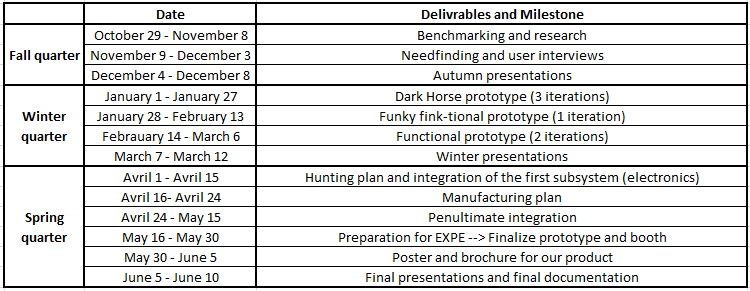
\includegraphics[scale=0.8]{images/planning.png}
   \caption{Deliverables and Milestones for the whole project}
  \label{fig:planning}
\end{figure}


\section{Distributed team management}

Over the past three quarters ,the seven of us have learned a lot of lessons about how to work together as a distributed team and how to take advantage of our diverse talents. Our diverse backgrounds (two mechanical engineers, one aerospace engineer, one product designer, two industrial engineers and one electrical engineer) allowed each of us to shine in various ways. During winter and spring quarter we challenged each other to take on something outside of our individual comfort zones, a challenge that brought with it some successes and some failures…\\

In order to ensure successful cooperation within the whole team, we decided to set a weekly meeting for the Winter and Spring quarters with our global partners. We found it was a very useful update on what each entity of the team had worked on during the week. It was also a valuable safety net when the schedule started to get very busy. In addition to these regular meetings, we also shared our documentation and our work on a Podio platform as well as on Google Drive. It enabled us to share content and react almost immediately to our peers’ ideas. When discussions were required between individuals who were collaborating, we used Skype as an informal and easy way to share ideas.\\

We believed that another attribute of our success as a team is the relationship that we built during the Stanford’s team visit to USP in March. The social connection and a good understanding allowed us to feel comfortable both to tease each other and to throw out crazy ideas which challenged the group.


\section{Project Budget}

\subsection{Stanford Budget}

\subsection{USP Budget}
 
\section{Reflection and Goals}

\subsection{Stanford Team}

\subsubsection{Clifford Bargar}

\subsubsection{Maria Barrera}
I first decided I wanted to take ME310 when I went to EXPE last year. I saw all of these production-quality prototypes in booths that looked so professional and, frankly, I was blown away. I knew then that I needed to be a part of this experience. It wasn't until midway through Fall Quarter, however, that I truly began to see the challenges that would unfold as our project moved forward.

They say the team is the most important part in a group project. Based on my experience, I could not agree more. Our team here at Stanford broke down a couple of times - ME310 is not a class that should be taken lightly and it is simply too much for some to handle. This obviously affected our progress as it was extremely hard to move forward when there were so many unresolved team issues. We were extremely lucky that our colleagues at USP were extremely passionate and hardworking, despite being a part of ME310 for the first time and not really knowing what the class would entail. They have been an amazing driving force for this team and I believe we, the Stanford team, owe a lot of our success to the USP students and their supportive teaching team.

We stated earlier that one of the things that we attribute to our success is the team bonding that occurred while the Stanford team was visiting USP. I wonder if we had done this earlier, or maybe taken the time to forge those types of relationship with the Stanford team early on, if our team troubles would have been less intense. This team experience is one I will never forget and will carry with me throughout my professional career. While I definitely believed I gained and refined ME-related skills, the most rewarding part of this class by far has been learning how to be a better team player and better leader. I know I still have a lot to improve but I am grateful for the opportunity to develop these skills in the confines of such an amazing class. 

I also could not be prouder of our EXPE booth- we killed it  :)

\subsubsection{Laura Hoinville}

This project was a great experience. I must admit it took me some time to understand what the expectations both from the class and from our users were. ME 310 was my first product design class and it made me realize how important it is to understand who your user is and how to put yourself in their shoes to make sure you your solution addresses their real problems. This project was a great opportunity to merge my engineering skills (I’m from an aerospace engineering background) with empathy and understanding of the needs and issues of people we were designing for.\\

I know a lot of aircraft design because this is the field where I’d like to start my career, but anytime I was taught about it, it was mainly in terms of aircraft performance and never in terms of people’s need. I think this project enabled me to see aircraft design from the user’s point of view instead of the aircraft manufacturer’s point of view and for me this was extremely valuable.//
Since I come from France it was actually the first time that I had the opportunity to work with both American and Brazilian people and this cultural diversity was also a great source of enrichment.\\

But beyond this, this project now means a lot to me. I got the opportunity to talk to disabled people and understand how painful it is for them to travel. They care a lot about our project because they see it as a way to improve their experience and I did not want to disappoint them. They deserve the right to enjoy their flights the way we do and for this reason I’m very excited to see what Embraer will do with our prototype and our work and I hope this will contribute in making the flying experience more enjoyable for people with reduced mobility. 


\subsection{USP Team}

\subsubsection{Luiz Durao}

        	When the project started 9 months ago, I was concerned about the direction we would take and the impact on the users' live we could create if we used our ideas correctly. As the time went by and we got closer to our user, I realized that their current experience is really bad and that really motivated to work toward a product that could truly be useful for people with reduced mobility. With that in mind, we developed a complex needfinding analysis, which made me see how difficult the life of people with reduced mobility truly is and how few solutions exists in this field. As the innovation process went by, I realized the importance of the teamwork and the importance of this brainstorming technique that opened our minds to problems that we, by ourselves, could not have thought about. The development of the dark horse prototype helped us consider an idea that was previously discarded by the group. For me, this was important as it gave new insights to the final product and helped push us along by showing us that we can’t design for all groups of people with reduced mobility since they have particular problems that increase the difficulty of universal design. Both functional and funktional prototypes were important in showing me that we had a direction to follow and that we were working hard to solve some important problems for our users.  The EXPE preparation was intense and surprisingly, showed me my ability to work under pressure. The results were great and I really enjoyed the feedback we got from our booth. As for working with an the international team, I must admit it was a bit of challenge at first to develop a good rhythm, but once we started working together we got a great result.

\subsubsection{Guilherme Kok}

\subsubsection{Rodrigo Monteiro}

At the the beginning of the project I thought it would be really difficult to develop a solution that could be satisfactory to our user's needs. But after talking to potential users and  going through numerous brainstorm sessions with the team, I was convinced that we would be able build a solution that could make the flight experience better for disabled passengers.

Building the prototype was challenging, expecially since we didn't have much experience buying tools and materials. But we managed to work through the limitations of materials and knowledge to build our final prototype.

It was great to see people's positive reaction to our prototype at EXPE. It was especially rewarding when Jose Luis Naranjo, who had advised and helped our team during the project, tested our redesigned aisle wheelchair.

Overall, the experiences that I acquired from this project is invaluable, and I'm happy that the result was well received.

\subsubsection{Amanda Mota}

The project began with a challenge: working within a restrictive environment such as the plane with a user who needs extra care. The search for how to improve our user's experience was a pleasant challenge to overcome. We saw a wide range of possibilities over the 9 months and it was very satisfying to see the different tests and prototypes.

All these months of work contributed to learning how airplanes and airline operate, as well as learning about seating, comfort and truly understanding the needs of our user. There was also a lot of group work, understanding of different areas of knowledge, and learning how to effectively use design to communicate. Finally, I was happy that able to improve my English.

The ultimate experience of working the last two weeks at Stanford was especially unforgettable. The preceding EXPE work made me work in a new environment with greater integration between the group and learning to deal with pressure of delivery and final presentation. As a final result my expectations were exceeded by what we delivered. We received great feedback from people who saw our project and that to me was very satisyinf; it made me proud and happy.

